% Options for packages loaded elsewhere
\PassOptionsToPackage{unicode}{hyperref}
\PassOptionsToPackage{hyphens}{url}
\PassOptionsToPackage{dvipsnames,svgnames,x11names}{xcolor}
%
\documentclass[
  letterpaper,
  DIV=11,
  numbers=noendperiod]{scrartcl}

\usepackage{amsmath,amssymb}
\usepackage{iftex}
\ifPDFTeX
  \usepackage[T2A]{fontenc}
  \usepackage[utf8]{inputenc}
  \usepackage{textcomp} % provide euro and other symbols
\else % if luatex or xetex
  \usepackage{unicode-math}
  \defaultfontfeatures{Scale=MatchLowercase}
  \defaultfontfeatures[\rmfamily]{Ligatures=TeX,Scale=1}
\fi
\usepackage{lmodern}
\ifPDFTeX\else  
    % xetex/luatex font selection
  \setmainfont[]{CMU Serif}
  \setsansfont[]{CMU Serif}
  \setmonofont[]{CMU Serif}
\fi
% Use upquote if available, for straight quotes in verbatim environments
\IfFileExists{upquote.sty}{\usepackage{upquote}}{}
\IfFileExists{microtype.sty}{% use microtype if available
  \usepackage[]{microtype}
  \UseMicrotypeSet[protrusion]{basicmath} % disable protrusion for tt fonts
}{}
\makeatletter
\@ifundefined{KOMAClassName}{% if non-KOMA class
  \IfFileExists{parskip.sty}{%
    \usepackage{parskip}
  }{% else
    \setlength{\parindent}{0pt}
    \setlength{\parskip}{6pt plus 2pt minus 1pt}}
}{% if KOMA class
  \KOMAoptions{parskip=half}}
\makeatother
\usepackage{xcolor}
\setlength{\emergencystretch}{3em} % prevent overfull lines
\setcounter{secnumdepth}{-\maxdimen} % remove section numbering
% Make \paragraph and \subparagraph free-standing
\ifx\paragraph\undefined\else
  \let\oldparagraph\paragraph
  \renewcommand{\paragraph}[1]{\oldparagraph{#1}\mbox{}}
\fi
\ifx\subparagraph\undefined\else
  \let\oldsubparagraph\subparagraph
  \renewcommand{\subparagraph}[1]{\oldsubparagraph{#1}\mbox{}}
\fi


\providecommand{\tightlist}{%
  \setlength{\itemsep}{0pt}\setlength{\parskip}{0pt}}\usepackage{longtable,booktabs,array}
\usepackage{calc} % for calculating minipage widths
% Correct order of tables after \paragraph or \subparagraph
\usepackage{etoolbox}
\makeatletter
\patchcmd\longtable{\par}{\if@noskipsec\mbox{}\fi\par}{}{}
\makeatother
% Allow footnotes in longtable head/foot
\IfFileExists{footnotehyper.sty}{\usepackage{footnotehyper}}{\usepackage{footnote}}
\makesavenoteenv{longtable}
\usepackage{graphicx}
\makeatletter
\def\maxwidth{\ifdim\Gin@nat@width>\linewidth\linewidth\else\Gin@nat@width\fi}
\def\maxheight{\ifdim\Gin@nat@height>\textheight\textheight\else\Gin@nat@height\fi}
\makeatother
% Scale images if necessary, so that they will not overflow the page
% margins by default, and it is still possible to overwrite the defaults
% using explicit options in \includegraphics[width, height, ...]{}
\setkeys{Gin}{width=\maxwidth,height=\maxheight,keepaspectratio}
% Set default figure placement to htbp
\makeatletter
\def\fps@figure{htbp}
\makeatother

\KOMAoption{captions}{tablesignature}
\usepackage[authordate, abbreviate = true, date = year, autocite=inline, backref = true]{biblatex-chicago}
\usepackage{csquotes}
\setlength{\bibhang}{0pt}
\makeatletter
\makeatother
\makeatletter
\makeatother
\makeatletter
\@ifpackageloaded{caption}{}{\usepackage{caption}}
\AtBeginDocument{%
\ifdefined\contentsname
  \renewcommand*\contentsname{Table of contents}
\else
  \newcommand\contentsname{Table of contents}
\fi
\ifdefined\listfigurename
  \renewcommand*\listfigurename{List of Figures}
\else
  \newcommand\listfigurename{List of Figures}
\fi
\ifdefined\listtablename
  \renewcommand*\listtablename{List of Tables}
\else
  \newcommand\listtablename{List of Tables}
\fi
\ifdefined\figurename
  \renewcommand*\figurename{Figure}
\else
  \newcommand\figurename{Figure}
\fi
\ifdefined\tablename
  \renewcommand*\tablename{Table}
\else
  \newcommand\tablename{Table}
\fi
}
\@ifpackageloaded{float}{}{\usepackage{float}}
\floatstyle{ruled}
\@ifundefined{c@chapter}{\newfloat{codelisting}{h}{lop}}{\newfloat{codelisting}{h}{lop}[chapter]}
\floatname{codelisting}{Listing}
\newcommand*\listoflistings{\listof{codelisting}{List of Listings}}
\makeatother
\makeatletter
\@ifpackageloaded{caption}{}{\usepackage{caption}}
\@ifpackageloaded{subcaption}{}{\usepackage{subcaption}}
\makeatother
\makeatletter
\@ifpackageloaded{tcolorbox}{}{\usepackage[skins,breakable]{tcolorbox}}
\makeatother
\makeatletter
\@ifundefined{shadecolor}{\definecolor{shadecolor}{rgb}{.97, .97, .97}}
\makeatother
\makeatletter
\makeatother
\makeatletter
\makeatother
\ifLuaTeX
\usepackage[bidi=basic]{babel}
\else
\usepackage[bidi=default]{babel}
\fi
\babelprovide[main,import]{english}
% get rid of language-specific shorthands (see #6817):
\let\LanguageShortHands\languageshorthands
\def\languageshorthands#1{}
\ifLuaTeX
  \usepackage{selnolig}  % disable illegal ligatures
\fi
\usepackage[]{biblatex}
\addbibresource{bibliography.bib}
\usepackage{csquotes}
\IfFileExists{bookmark.sty}{\usepackage{bookmark}}{\usepackage{hyperref}}
\IfFileExists{xurl.sty}{\usepackage{xurl}}{} % add URL line breaks if available
\urlstyle{same} % disable monospaced font for URLs
\hypersetup{
  pdftitle={Student dropout analysis based on previously acquired educational achievements: A case of the University of Portalegre},
  pdfauthor={Izeldeen Nedal Yunis Al Fraijat; Danat Semeneev; Ieva Žube; Pankaj Chattri; Kristaps Eglītis},
  pdflang={en},
  pdfkeywords={AA1, AA2},
  colorlinks=true,
  linkcolor={blue},
  filecolor={Maroon},
  citecolor={Blue},
  urlcolor={Blue},
  pdfcreator={LaTeX via pandoc}}

\title{Student dropout analysis based on previously acquired educational
achievements: A case of the University of Portalegre}
\usepackage{etoolbox}
\makeatletter
\providecommand{\subtitle}[1]{% add subtitle to \maketitle
  \apptocmd{\@title}{\par {\large #1 \par}}{}{}
}
\makeatother
\subtitle{Business Analysis, Business Informatics Ms, Fall 2023.}
\author{Izeldeen Nedal Yunis Al Fraijat \and Danat Semeneev \and Ieva
Žube \and Pankaj Chattri \and Kristaps Eglītis\footnote{Rīga Technical
  University}}
\date{2023-12-11}

\begin{document}
\maketitle
\begin{abstract}
.
\end{abstract}
\ifdefined\Shaded\renewenvironment{Shaded}{\begin{tcolorbox}[borderline west={3pt}{0pt}{shadecolor}, breakable, interior hidden, enhanced, sharp corners, boxrule=0pt, frame hidden]}{\end{tcolorbox}}\fi

\hypertarget{abstract}{%
\subsection{Abstract}\label{abstract}}

In the world of education, the path to success is often visualized as a
linear progression, where students follow a predefined journey from
kindergarten to graduation. However, the reality is far more complex.
Various reasons lead students to choose to deviate from this path. These
students have encountered different challenges, circumstances, or a lack
of proper resources that have led them to drop out of university.

In this dataset provided to us, we will delve deeper into understanding
the reasons why students have dropped out of the university, based on
the data at our disposal. We will leverage our social knowledge to
comprehend the factors that influenced their decision to drop out and
work to prevent such occurrences if the issues are within the
university's purview. Our goal is to offer solutions, support, and the
necessary resources to facilitate students' educational journeys. We
will also use the analysis we've conducted on the dropout students to
learn from their experiences and chart a unique educational pathway with
fewer dropouts.

\hypertarget{introduction}{%
\section{Introduction}\label{introduction}}

Starting from preliminary school we are told that having an education is
very important for your future or that without higher education your job
possibilities are going to be very limited. While primary education is
mandatory, having higher education is not. But why do people actually
take their time and resources to pursue it? Well, according to studies
the most important factor for pursuing higher education is job
acquisition. \autocite{knutsen_motivation_2011} Some other factors may
include increased income in the existing job, improved work conditions
or increased ability for retirement. All in all they do all tie up to
materialistic benefits in the end. Of course, other, more intrisic
factors include seeking for additional knowledge or self-fulfillment
\autocite{cortes_factors_2023}. There are also factors like meeting new
friends, improving social interaction skills or just wanting to make a
difference in the world. Of course factors that cannot be ignored are
social pressure \autocite{temple_factors_2009}, meaning that having
friends that want to pursue higher education can influence ones own
decision or influence of family members. Pursuing higher edication is
good, but what about people who prematurely end their studies and drop
out? What could be the factors that lead to such a decision? Based on
the study and datasets that we used for our research there are multiple
factors that influence dropping out.

Nevertheless, pursuing higher education and actually getting the degree
has some tangible benefits. According to an OECD -- Education at a
Glance 2019 research paper \autocite{oecd_education_2019}, \enquote{On
average across OECD countries, adults with a short-cycle tertiary degree
earn 20\% more than adults with upper secondary education. The earnings
advantage increases to 44\% for those with a bachelor's degree and to
91\% for those with a master's or doctorPal degree.} With this in mind,
it is important for government and educational institutions to ensure
high level of graduates in society to ensure economic growth and overall
increase in well-being. To measure the success of this goal, it is
important to set KPI's, track them and make educated conclusions on what
needs to be done or is being done right to reach the goal of higher
educated society.

\hypertarget{target-metrics-and-kpi}{%
\subsection{Target Metrics and KPI}\label{target-metrics-and-kpi}}

In this particular case, KPI's will be chosen based on datasets of
Portugese High Schools but most likely data can be generalised, atleast
for Europe, as the region and sociodemographics are not so different.
Even though there are many factors that influence the success of
graduation, only factors that can be proven by government and
educational institutions will be chosen. After rigorous analysis, we
propose the following grades.

\begin{enumerate}
\def\labelenumi{\arabic{enumi}.}
\item
  Academic support. Based on the dataset students who had support had 3x
  lower dropout rates than students that didn't have. This means that
  governments should be incentivised to allocate a higher amount of
  budget towards education to give financial aid and motivate students
  to complete their studies.
\item
  Institutional improvements. Again, based on datasets, schools with
  improvements have 40\% less dropout rate than schools without. This is
  something that can be improved by incentivizing teachers with higher
  salaries or giving schools more budget to improve their workstations.
\item
  Student grades. Datasets tell us that the higher the average grade,
  the lower the dropout rate. Usually students that have low grades are
  uninterested in the subjects which could be due to having chosen not
  the right program for them or that the way lectures and information is
  presented is uninteresting or outdated. Either way this can be
  improved. Increasing the possibility that the student has chosen the
  right program for him can be done by introducing more \enquote{open
  days} in higher education institutions and having more upfront
  information about what can be expected from programs. The overall
  lecture performance can be improved by taking more time to have
  up-to-date information presented and teachers having decent motivation
  of teaching students. This can be achieved by increasing teacher
  salaries and institutions having more control over teachers and
  information they present to students.
\end{enumerate}

\hypertarget{exploratory-data-analysis}{%
\subsection{Exploratory Data Analysis}\label{exploratory-data-analysis}}

\hypertarget{descriptive-statistics}{%
\subsubsection{Descriptive Statistics}\label{descriptive-statistics}}

\hypertarget{tab-example}{}
\begin{longtable}[]{@{}ll@{}}
\toprule\noalign{}
& Data Type \\
\midrule\noalign{}
\endfirsthead
\toprule\noalign{}
& Data Type \\
\midrule\noalign{}
\endhead
\bottomrule\noalign{}
\endlastfoot
Marital status & int64 \\
Application mode & int64 \\
Application order & int64 \\
Course & int64 \\
Daytime/evening attendance & int64 \\
Previous qualification & int64 \\
Previous qualification (grade) & float64 \\
Nacionality & int64 \\
Mother\textquotesingle s qualification & int64 \\
Father\textquotesingle s qualification & int64 \\
Mother\textquotesingle s occupation & int64 \\
Father\textquotesingle s occupation & int64 \\
Admission grade & float64 \\
Displaced & int64 \\
Educational special needs & int64 \\
Debtor & int64 \\
Tuition fees up to date & int64 \\
Gender & int64 \\
Scholarship holder & int64 \\
Age at enrollment & int64 \\
International & int64 \\
Curricular units 1st sem (credited) & int64 \\
Curricular units 1st sem (enrolled) & int64 \\
Curricular units 1st sem (evaluations) & int64 \\
Curricular units 1st sem (approved) & int64 \\
Curricular units 1st sem (grade) & float64 \\
Curricular units 1st sem (without evaluations) & int64 \\
Curricular units 2nd sem (credited) & int64 \\
Curricular units 2nd sem (enrolled) & int64 \\
Curricular units 2nd sem (evaluations) & int64 \\
Curricular units 2nd sem (approved) & int64 \\
Curricular units 2nd sem (grade) & float64 \\
Curricular units 2nd sem (without evaluations) & int64 \\
Unemployment rate & float64 \\
Inflation rate & float64 \\
GDP & float64 \\
Target & object \\
\caption{The data types of the datast columns }\tabularnewline
\end{longtable}

As we have checked, the dataset does not have zero values, so there is
nothing to purge inside it. Later on, we get the basic descriptive
statistics, shown below.

\hypertarget{tab-descstat-1}{}
\begin{longtable}[]{@{}llllll@{}}
\toprule\noalign{}
& Marital status & Application mode & Application order & Course &
Daytime/evening attendance \\
\midrule\noalign{}
\endfirsthead
\toprule\noalign{}
& Marital status & Application mode & Application order & Course &
Daytime/evening attendance \\
\midrule\noalign{}
\endhead
\bottomrule\noalign{}
\endlastfoot
count & 4424.00 & 4424.00 & 4424.00 & 4424.00 & 4424.00 \\
mean & 1.18 & 18.67 & 1.73 & 8856.64 & 0.89 \\
std & 0.61 & 17.48 & 1.31 & 2063.57 & 0.31 \\
min & 1.00 & 1.00 & 0.00 & 33.00 & 0.00 \\
25\% & 1.00 & 1.00 & 1.00 & 9085.00 & 1.00 \\
50\% & 1.00 & 17.00 & 1.00 & 9238.00 & 1.00 \\
75\% & 1.00 & 39.00 & 2.00 & 9556.00 & 1.00 \\
max & 6.00 & 57.00 & 9.00 & 9991.00 & 1.00 \\
\caption{Descriptive statistics }\tabularnewline
\end{longtable}

\hypertarget{tab-descstat-2}{}
\begin{longtable}[]{@{}llllll@{}}
\toprule\noalign{}
& Previous qualification & Previous qualification (grade) & Nacionality
& Mother\textquotesingle s qualification & Father\textquotesingle s
qualification \\
\midrule\noalign{}
\endfirsthead
\toprule\noalign{}
& Previous qualification & Previous qualification (grade) & Nacionality
& Mother\textquotesingle s qualification & Father\textquotesingle s
qualification \\
\midrule\noalign{}
\endhead
\bottomrule\noalign{}
\endlastfoot
count & 4424.00 & 4424.00 & 4424.00 & 4424.00 & 4424.00 \\
mean & 4.58 & 132.61 & 1.87 & 19.56 & 22.28 \\
std & 10.22 & 13.19 & 6.91 & 15.60 & 15.34 \\
min & 1.00 & 95.00 & 1.00 & 1.00 & 1.00 \\
25\% & 1.00 & 125.00 & 1.00 & 2.00 & 3.00 \\
50\% & 1.00 & 133.10 & 1.00 & 19.00 & 19.00 \\
75\% & 1.00 & 140.00 & 1.00 & 37.00 & 37.00 \\
max & 43.00 & 190.00 & 109.00 & 44.00 & 44.00 \\
\caption{Descriptive statistics (cont'd) }\tabularnewline
\end{longtable}

\hypertarget{tab-descstat-3}{}
\begin{longtable}[]{@{}llllll@{}}
\toprule\noalign{}
& Mother\textquotesingle s occupation & Father\textquotesingle s
occupation & Admission grade & Displaced & Educational special needs \\
\midrule\noalign{}
\endfirsthead
\toprule\noalign{}
& Mother\textquotesingle s occupation & Father\textquotesingle s
occupation & Admission grade & Displaced & Educational special needs \\
\midrule\noalign{}
\endhead
\bottomrule\noalign{}
\endlastfoot
count & 4424.00 & 4424.00 & 4424.00 & 4424.00 & 4424.00 \\
mean & 10.96 & 11.03 & 126.98 & 0.55 & 0.01 \\
std & 26.42 & 25.26 & 14.48 & 0.50 & 0.11 \\
min & 0.00 & 0.00 & 95.00 & 0.00 & 0.00 \\
25\% & 4.00 & 4.00 & 117.90 & 0.00 & 0.00 \\
50\% & 5.00 & 7.00 & 126.10 & 1.00 & 0.00 \\
75\% & 9.00 & 9.00 & 134.80 & 1.00 & 0.00 \\
max & 194.00 & 195.00 & 190.00 & 1.00 & 1.00 \\
\caption{Descriptive statistics (cont'd) }\tabularnewline
\end{longtable}

\hypertarget{tab-descstat-4}{}
\begin{longtable}[]{@{}llllll@{}}
\toprule\noalign{}
& Debtor & Tuition fees up to date & Gender & Scholarship holder & Age
at enrollment \\
\midrule\noalign{}
\endfirsthead
\toprule\noalign{}
& Debtor & Tuition fees up to date & Gender & Scholarship holder & Age
at enrollment \\
\midrule\noalign{}
\endhead
\bottomrule\noalign{}
\endlastfoot
count & 4424.00 & 4424.00 & 4424.00 & 4424.00 & 4424.00 \\
mean & 0.11 & 0.88 & 0.35 & 0.25 & 23.27 \\
std & 0.32 & 0.32 & 0.48 & 0.43 & 7.59 \\
min & 0.00 & 0.00 & 0.00 & 0.00 & 17.00 \\
25\% & 0.00 & 1.00 & 0.00 & 0.00 & 19.00 \\
50\% & 0.00 & 1.00 & 0.00 & 0.00 & 20.00 \\
75\% & 0.00 & 1.00 & 1.00 & 0.00 & 25.00 \\
max & 1.00 & 1.00 & 1.00 & 1.00 & 70.00 \\
\caption{Descriptive statistics (cont'd) }\tabularnewline
\end{longtable}

\hypertarget{tab-descstat-5}{}
\begin{longtable}[]{@{}lllll@{}}
\toprule\noalign{}
& International & Curricular units 1st sem (credited) & Curricular units
1st sem (enrolled) & Curricular units 1st sem (evaluations) \\
\midrule\noalign{}
\endfirsthead
\toprule\noalign{}
& International & Curricular units 1st sem (credited) & Curricular units
1st sem (enrolled) & Curricular units 1st sem (evaluations) \\
\midrule\noalign{}
\endhead
\bottomrule\noalign{}
\endlastfoot
count & 4424.00 & 4424.00 & 4424.00 & 4424.00 \\
mean & 0.02 & 0.71 & 6.27 & 8.30 \\
std & 0.16 & 2.36 & 2.48 & 4.18 \\
min & 0.00 & 0.00 & 0.00 & 0.00 \\
25\% & 0.00 & 0.00 & 5.00 & 6.00 \\
50\% & 0.00 & 0.00 & 6.00 & 8.00 \\
75\% & 0.00 & 0.00 & 7.00 & 10.00 \\
max & 1.00 & 20.00 & 26.00 & 45.00 \\
\caption{Descriptive statistics (cont'd) }\tabularnewline
\end{longtable}

\hypertarget{tab-descstat-6}{}
\begin{longtable}[]{@{}lllll@{}}
\toprule\noalign{}
& Curricular units 1st sem (approved) & Curricular units 1st sem (grade)
& Curricular units 1st sem (without evaluations) & Curricular units 2nd
sem (credited) \\
\midrule\noalign{}
\endfirsthead
\toprule\noalign{}
& Curricular units 1st sem (approved) & Curricular units 1st sem (grade)
& Curricular units 1st sem (without evaluations) & Curricular units 2nd
sem (credited) \\
\midrule\noalign{}
\endhead
\bottomrule\noalign{}
\endlastfoot
count & 4424.00 & 4424.00 & 4424.00 & 4424.00 \\
mean & 4.71 & 10.64 & 0.14 & 0.54 \\
std & 3.09 & 4.84 & 0.69 & 1.92 \\
min & 0.00 & 0.00 & 0.00 & 0.00 \\
25\% & 3.00 & 11.00 & 0.00 & 0.00 \\
50\% & 5.00 & 12.29 & 0.00 & 0.00 \\
75\% & 6.00 & 13.40 & 0.00 & 0.00 \\
max & 26.00 & 18.88 & 12.00 & 19.00 \\
\caption{Descriptive statistics (cont'd) }\tabularnewline
\end{longtable}

\hypertarget{tab-descstat-7}{}
\begin{longtable}[]{@{}lllll@{}}
\toprule\noalign{}
& Curricular units 2nd sem (enrolled) & Curricular units 2nd sem
(evaluations) & Curricular units 2nd sem (approved) & Curricular units
2nd sem (grade) \\
\midrule\noalign{}
\endfirsthead
\toprule\noalign{}
& Curricular units 2nd sem (enrolled) & Curricular units 2nd sem
(evaluations) & Curricular units 2nd sem (approved) & Curricular units
2nd sem (grade) \\
\midrule\noalign{}
\endhead
\bottomrule\noalign{}
\endlastfoot
count & 4424.00 & 4424.00 & 4424.00 & 4424.00 \\
mean & 6.23 & 8.06 & 4.44 & 10.23 \\
std & 2.20 & 3.95 & 3.01 & 5.21 \\
min & 0.00 & 0.00 & 0.00 & 0.00 \\
25\% & 5.00 & 6.00 & 2.00 & 10.75 \\
50\% & 6.00 & 8.00 & 5.00 & 12.20 \\
75\% & 7.00 & 10.00 & 6.00 & 13.33 \\
max & 23.00 & 33.00 & 20.00 & 18.57 \\
\caption{Descriptive statistics (cont'd) }\tabularnewline
\end{longtable}

The students are from multiple countries, but the overwhelming majority
of the students are from Portugal. It would be interesting to see how
the students' admission grade depends on their previous qualification in
their home countries, but the samples are scarce. Many students from
abroad are from the Ultramarine Territories where it's more challenging
to get comparable education. However, they and inland Portugal students
were naturally given some exemptions, as the dataset states \footnote{Link
  to the dataset description:
  \url{https://archive.ics.uci.edu/dataset/697/predict+students+dropout+and+academic+success}}

. For example, the students admitted per Ordance no. 854 \footnote{Link
  to the source document:
  \url{https://dre.tretas.org/dre/106607/portaria-854-B-99-de-4-de-outubro}}
were not required to demonstrate the proof of their validity since their
received a diploma in secondary education administered in Portuguese
(Angola, East Timor, Mozambique, Guinea Equatorial). Students admitted
per Ordnance no. 533 \footnote{Link to the source document:
  \url{https://dre.tretas.org/dre/104726/portaria-533-A-99-de-22-de-julho}}
were from another university in Portugal with overlapping courses
covered recently enough so they were not required to repeat them.
Finally, those admitted per Ord. no. 612 \footnote{Link to the source
  document:
  \url{https://dre.tretas.org/dre/51542/portaria-612-93-de-29-de-junho}}
came from other countries but had comparable material in their studies
and so their points were recalculated with some amortization.

\begin{figure}

{\centering 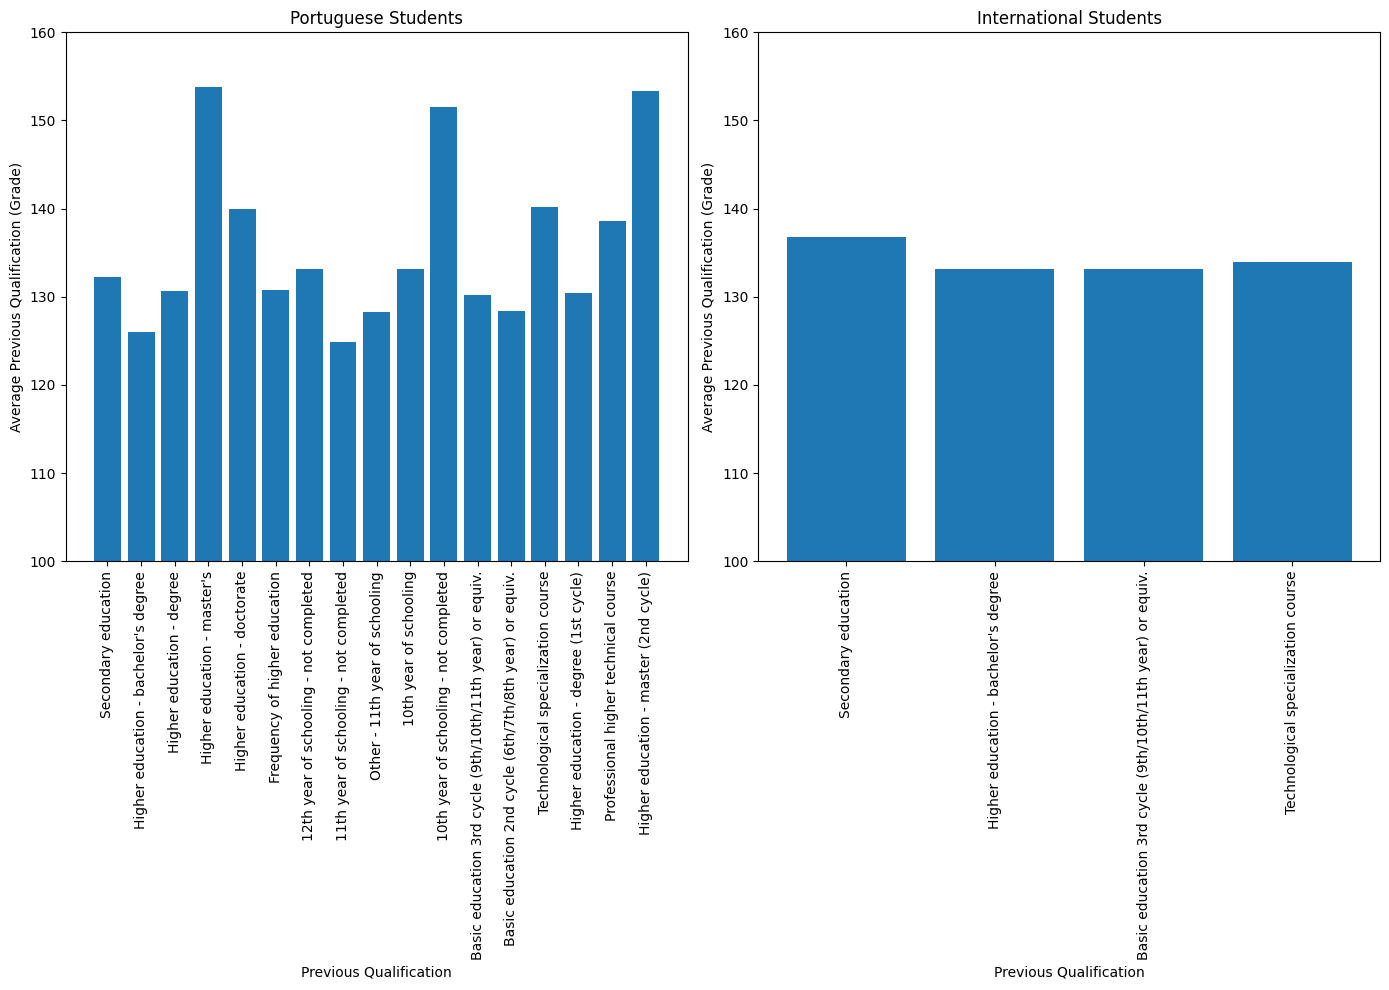
\includegraphics{report_AzadhdhinNedalYunisAlFraijat_files/figure-pdf/fig-education-output-1.png}

}

\caption{\label{fig-education}Relative graduation points for students
with different education backgrounds}

\end{figure}

Due to class imbalance , the variability for the Portuguese is much
higher, and while the 3 categories with highest grades are natural, i.
e. doctors, masters as higher education, the 3rd is unintuitive (the 10
classes) and we tend to explain it as self-selection and high
correlation with other indicators (those entering the university in the
10th grade are more motivated then dwelling in schools in 11th and 12th
grades).

Also, there is a drastic imbalance over yet another crucial factor: age.
As it was mentioned previously, students of age are far less ubiquitous,
can have far more incentives to abandon studies and with smaller
potential to apprehension of material. Indeed, this is eloquently
manifested on the next graph.

\begin{figure}

{\centering 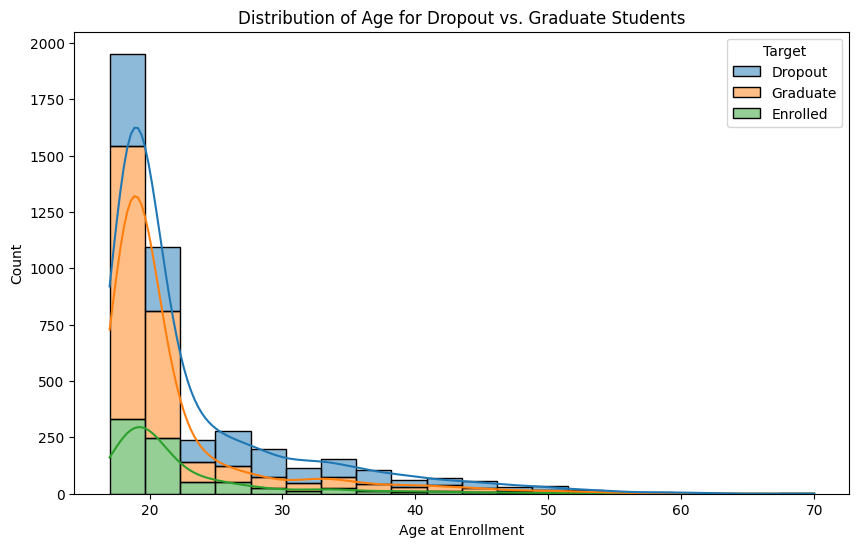
\includegraphics{report_AzadhdhinNedalYunisAlFraijat_files/figure-pdf/fig-age-distr-output-1.png}

}

\caption{\label{fig-age-distr}Distribution of age for dropout and
graduate student}

\end{figure}

Q. v. the sizes of the bins for dropout students differ far less than
the total size for the name of the student.

If the hypothesis about some external factors, The target variable
should be much dependent on previous grades,\\
The datapoint cloud, however, shows that this rule has a lot of
exceptions.

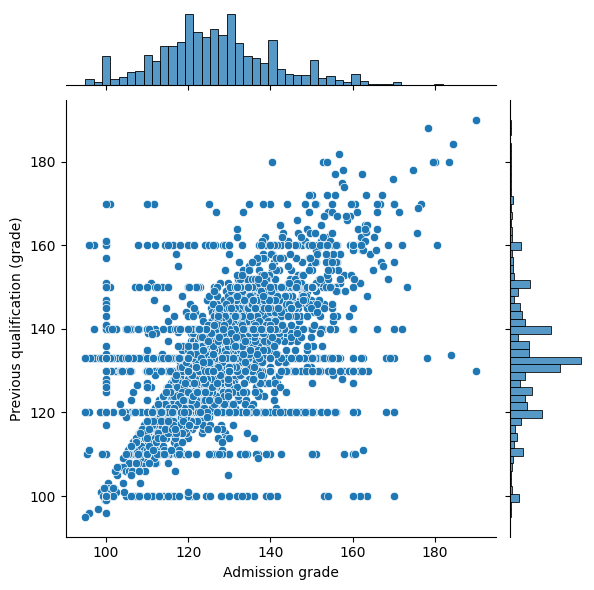
\includegraphics{report_AzadhdhinNedalYunisAlFraijat_files/figure-pdf/cell-22-output-1.png}

We can draw the following observations:

\begin{itemize}
\item
  The \textbf{distribution of admission grades} is roughly normal with
  most students scoring between \textbf{\emph{60 to 80 marks}}.
\item
  The \textbf{distribution of previous qualifications} (grades) is also
  the same with most of them having grades in between \textbf{\emph{12
  and 16}}.
\item
  There is seen a \textbf{positive correlation} between admission grade
  and previous qualification grade indicating students with higher
  previous qualifications tend to have higher admission grades.
\end{itemize}

This was the visualization for the few quantitative columns, which shows
the natural interconnection between the curricularly accrued units in
the 1st and the 2nd year, which are in turn mostly unrelated to the
admission grade. This is understandable since the grades are commonly
based on the successfulness of the local program and student's toil,
while the students' backgrounds are commonly different and this puts
them into inequitable positions when passing the admission exams.

In these previous graphs, we considered quantitative columns that are
more or less exogenous to the dataset (e. g. age and the previous
qualification grade are not influenced by the the current grade of the
students).

However, the majority of columns of this dataset are qualitative and
they are at least partially endogenous as stulk from the decisions
during the study. For this, we need to propose a mechanism of influence,
then formulate and test a hypothesis via an analysis of discriminate
groups.

We also consider the impact of scholarships and other compensations in
academic support, which should alleviate the complications associated
with adaptations in new environment.

\begin{figure}

{\centering 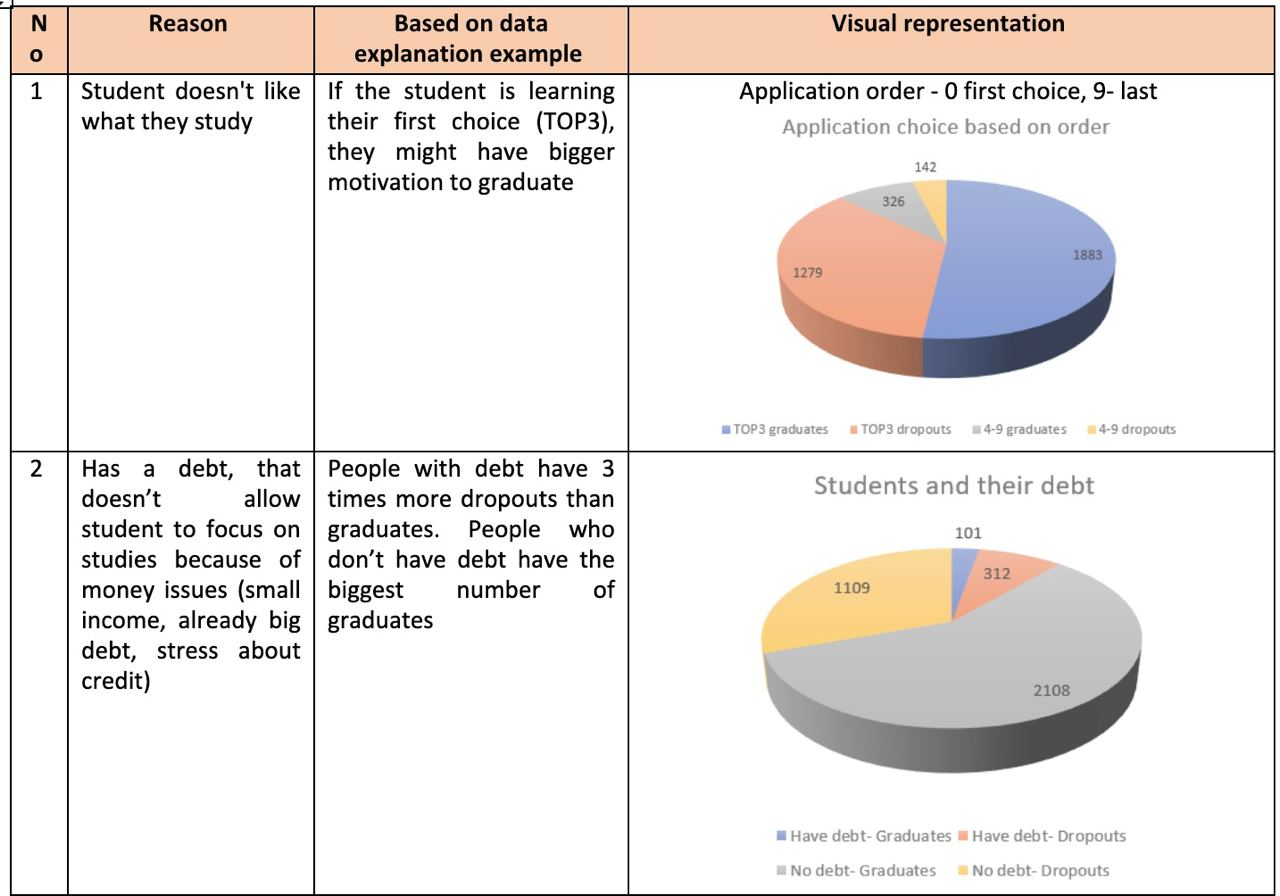
\includegraphics{./figs/reasons-1.jpg}

}

\caption{Student mobility and financial burden as indicators and drivers
of their motivation and impediments}

\end{figure}

We see that having debt is always a serious impediment against studies
because it gives wrong incentives towards directly making money in the
short run instead of mastering knowledge that could aid to make
altogether greater money in the long run.

\begin{figure}

{\centering 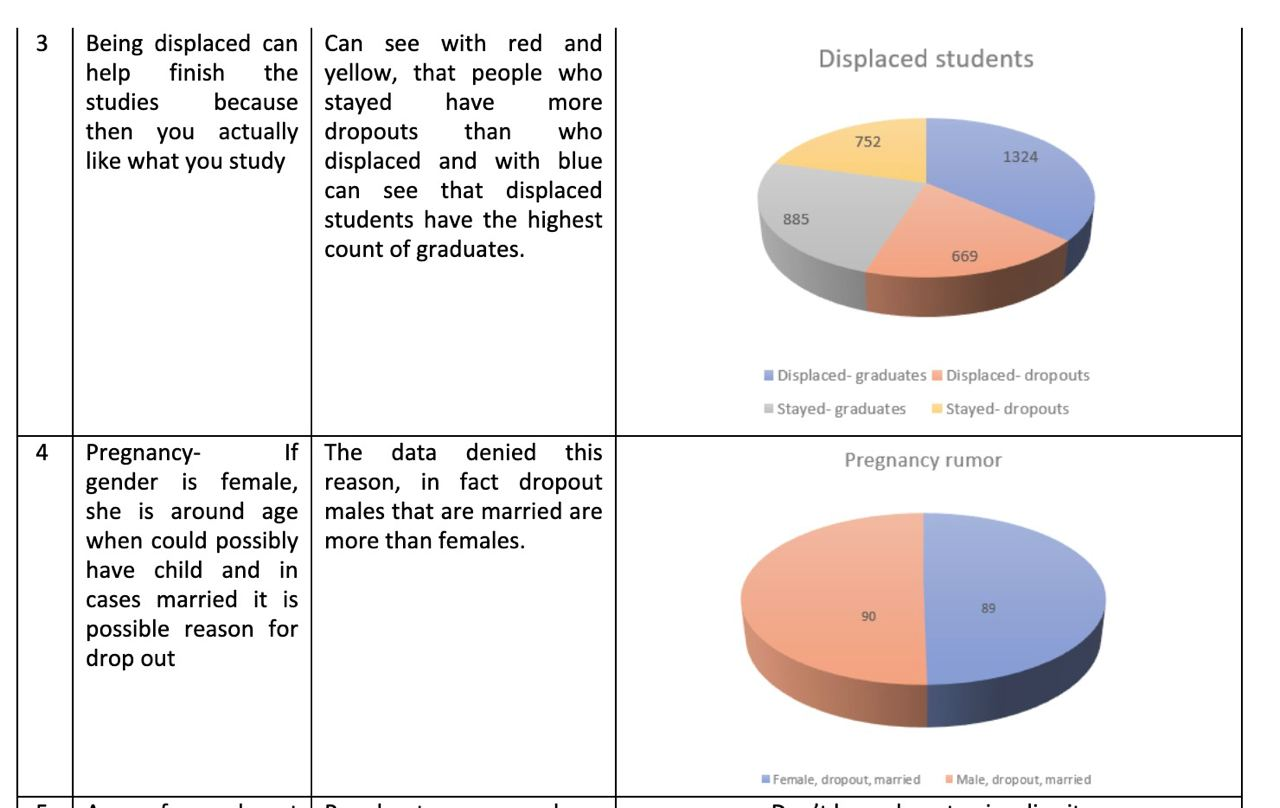
\includegraphics{./figs/reasons2.jpg}

}

\caption{Student inter-university mobility and health conditions proxies
as indicators and drivers of their motivation towards learning and
impediments (Part 2)}

\end{figure}

\begin{figure}

{\centering 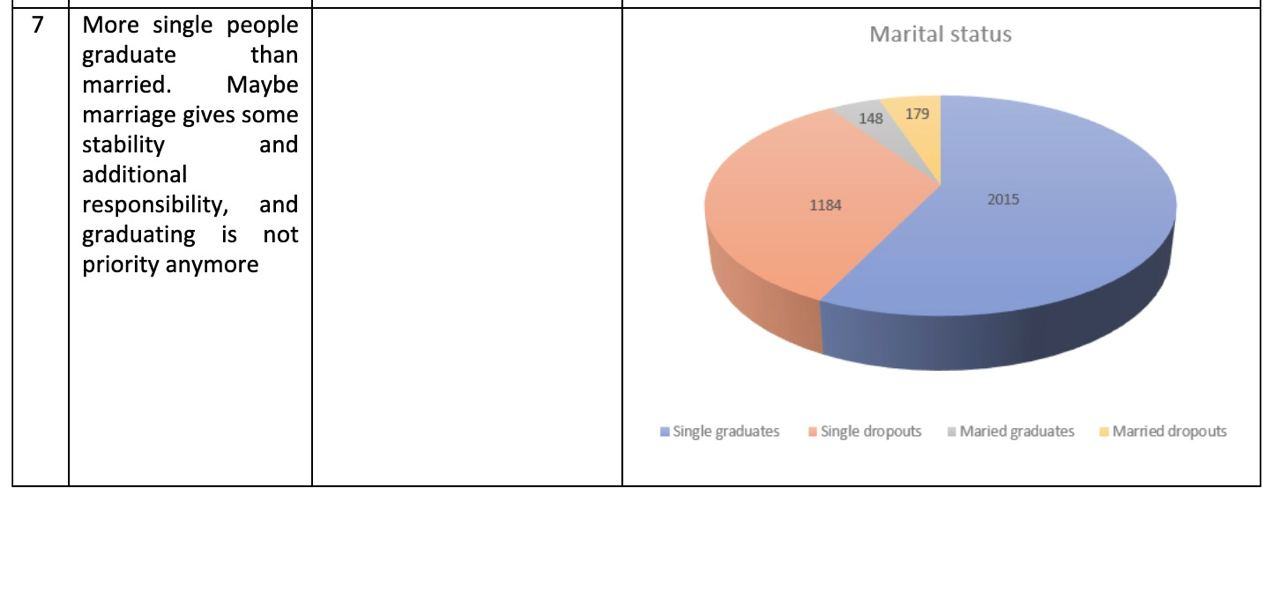
\includegraphics{./figs/rasons-3.jpg}

}

\caption{Marital status as distractor from studying}

\end{figure}

In different studies, it is quite common to compare the academic success
of a student with the academic successes of ttheir parents as this has
both direct and indirect effects , s. a. i. e. both are connected to
welfare, but also it can be that there is another channel of knowledge
transmission to the younger generation.

\textbf{Observations :} * The bar chart shows that mother's occupation
is quite influential. This influence is greater the pa's due to
traditional effect, and we distinctly see that students whose mothers
are \enquote*{white collars} dropout significantly more rarely than
those whose mothers are more engaged in physical labor.

\begin{itemize}
\tightlist
\item
  This also may suggest the mother's occupation can influence student
  retention, emphasizing the need for financial support and family
  engagement.
\end{itemize}

\hypertarget{data-correlation-table-quantitative-columns-only}{%
\subsubsection{Data correlation table (quantitative columns
only)}\label{data-correlation-table-quantitative-columns-only}}

\begin{figure}

{\centering 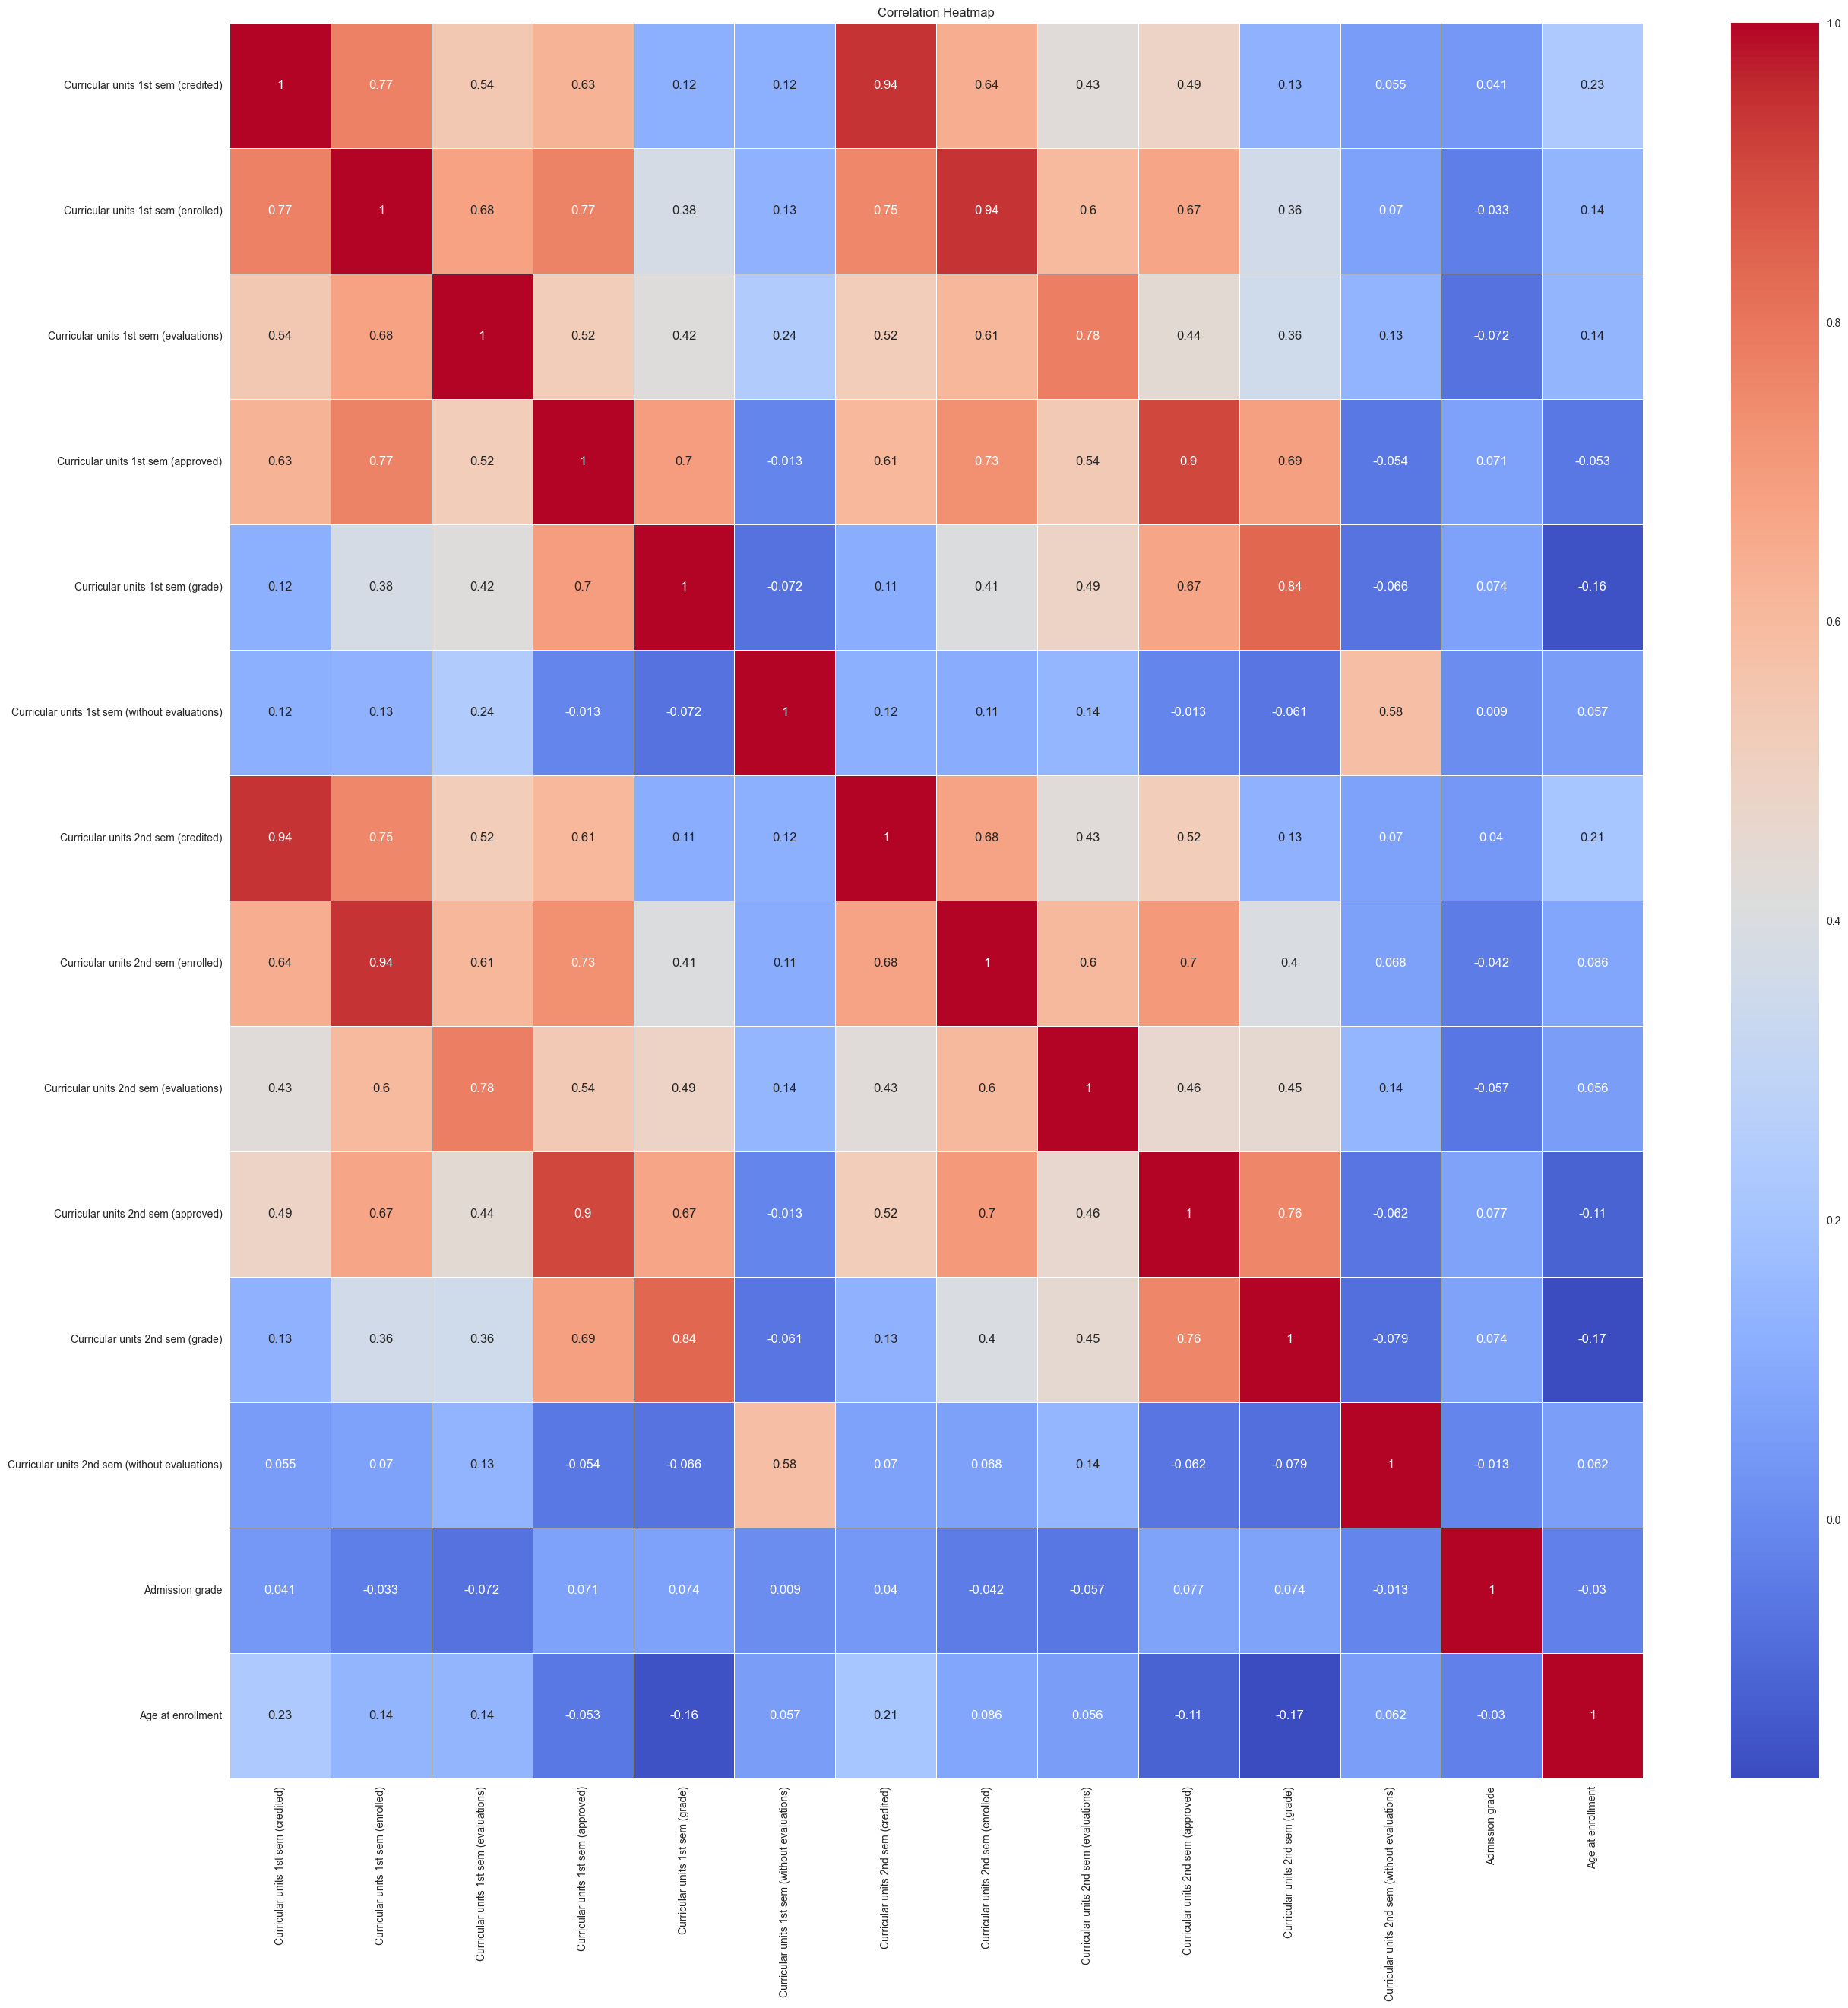
\includegraphics{report_AzadhdhinNedalYunisAlFraijat_files/figure-pdf/tab-correlation-output-1.png}

}

\caption{Data correlation table (quantitative columns are represented
only since there to compute true correlations between quantitative
columns it is necessary to OHE-encode them, which would burst no. of
columns to many thousands, but the values of the correlations will be
statistically insignificant due to low cardinality of 90\% of classes)}

\end{figure}

In this matrix for correlations, we already see high correlations
between many values. Hence, if we (certainly) consider qualitative
variables in our data mining analysis, we must reduce the number of
variables because the true dimensionality of the initial space is too
high and virtually all ways of embedding are too costly and prohibitive
given a relatively small amount of datapoints in this dataset. First our
common step would be to dispose of multicollinear columns.\\
High dimensionality prevents intuitive DBSCAN threshold setting and some
inferior algorithms as TSNE.

\begin{verbatim}
Index(['Marital status', 'Application mode', 'Application order', 'Course',
       'Daytime/evening attendance', 'Previous qualification',
       'Previous qualification (grade)', 'Nacionality',
       'Mother's qualification', 'Father's qualification',
       'Mother's occupation', 'Father's occupation', 'Admission grade',
       'Displaced', 'Educational special needs', 'Debtor',
       'Tuition fees up to date', 'Gender', 'Scholarship holder',
       'Age at enrollment', 'International',
       'Curricular units 1st sem (credited)',
       'Curricular units 1st sem (enrolled)',
       'Curricular units 1st sem (evaluations)',
       'Curricular units 1st sem (approved)',
       'Curricular units 1st sem (grade)',
       'Curricular units 1st sem (without evaluations)',
       'Curricular units 2nd sem (credited)',
       'Curricular units 2nd sem (enrolled)',
       'Curricular units 2nd sem (evaluations)',
       'Curricular units 2nd sem (approved)',
       'Curricular units 2nd sem (grade)',
       'Curricular units 2nd sem (without evaluations)', 'Unemployment rate',
       'Inflation rate', 'GDP', 'Target'],
      dtype='object')
\end{verbatim}

\begin{verbatim}
Found existing installation: pycaret 3.2.0
Uninstalling pycaret-3.2.0:
  Successfully uninstalled pycaret-3.2.0
\end{verbatim}

\begin{verbatim}
Collecting mlflow
  Using cached mlflow-2.9.1-py3-none-any.whl (19.1 MB)
Requirement already satisfied: click<9,>=7.0 in /opt/homebrew/Caskroom/miniconda/base/lib/python3.11/site-packages (from mlflow) (8.1.7)
Requirement already satisfied: cloudpickle<4 in /opt/homebrew/Caskroom/miniconda/base/lib/python3.11/site-packages (from mlflow) (3.0.0)
Requirement already satisfied: databricks-cli<1,>=0.8.7 in /opt/homebrew/Caskroom/miniconda/base/lib/python3.11/site-packages (from mlflow) (0.18.0)
Requirement already satisfied: entrypoints<1 in /opt/homebrew/Caskroom/miniconda/base/lib/python3.11/site-packages (from mlflow) (0.4)
Requirement already satisfied: gitpython<4,>=2.1.0 in /opt/homebrew/Caskroom/miniconda/base/lib/python3.11/site-packages (from mlflow) (3.1.40)
Requirement already satisfied: pyyaml<7,>=5.1 in /opt/homebrew/Caskroom/miniconda/base/lib/python3.11/site-packages (from mlflow) (6.0.1)
Requirement already satisfied: protobuf<5,>=3.12.0 in /opt/homebrew/Caskroom/miniconda/base/lib/python3.11/site-packages (from mlflow) (4.24.4)
Requirement already satisfied: pytz<2024 in /opt/homebrew/Caskroom/miniconda/base/lib/python3.11/site-packages (from mlflow) (2023.3.post1)
Requirement already satisfied: requests<3,>=2.17.3 in /opt/homebrew/Caskroom/miniconda/base/lib/python3.11/site-packages (from mlflow) (2.31.0)
Requirement already satisfied: packaging<24 in /opt/homebrew/Caskroom/miniconda/base/lib/python3.11/site-packages (from mlflow) (23.1)
Requirement already satisfied: importlib-metadata!=4.7.0,<8,>=3.7.0 in /opt/homebrew/Caskroom/miniconda/base/lib/python3.11/site-packages (from mlflow) (6.8.0)
Requirement already satisfied: sqlparse<1,>=0.4.0 in /opt/homebrew/Caskroom/miniconda/base/lib/python3.11/site-packages (from mlflow) (0.4.4)
Requirement already satisfied: alembic!=1.10.0,<2 in /opt/homebrew/Caskroom/miniconda/base/lib/python3.11/site-packages (from mlflow) (1.13.0)
Requirement already satisfied: docker<7,>=4.0.0 in /opt/homebrew/Caskroom/miniconda/base/lib/python3.11/site-packages (from mlflow) (6.1.3)
Requirement already satisfied: Flask<4 in /opt/homebrew/Caskroom/miniconda/base/lib/python3.11/site-packages (from mlflow) (3.0.0)
Requirement already satisfied: numpy<2 in /opt/homebrew/Caskroom/miniconda/base/lib/python3.11/site-packages (from mlflow) (1.25.2)
Requirement already satisfied: scipy<2 in /opt/homebrew/Caskroom/miniconda/base/lib/python3.11/site-packages (from mlflow) (1.10.1)
Requirement already satisfied: pandas<3 in /opt/homebrew/Caskroom/miniconda/base/lib/python3.11/site-packages (from mlflow) (1.5.3)
Requirement already satisfied: querystring-parser<2 in /opt/homebrew/Caskroom/miniconda/base/lib/python3.11/site-packages (from mlflow) (1.2.4)
Requirement already satisfied: sqlalchemy<3,>=1.4.0 in /opt/homebrew/Caskroom/miniconda/base/lib/python3.11/site-packages (from mlflow) (1.4.41)
Requirement already satisfied: scikit-learn<2 in /opt/homebrew/Caskroom/miniconda/base/lib/python3.11/site-packages (from mlflow) (1.2.2)
Requirement already satisfied: pyarrow<15,>=4.0.0 in /opt/homebrew/Caskroom/miniconda/base/lib/python3.11/site-packages (from mlflow) (12.0.1)
Requirement already satisfied: markdown<4,>=3.3 in /opt/homebrew/Caskroom/miniconda/base/lib/python3.11/site-packages (from mlflow) (3.5)
Requirement already satisfied: matplotlib<4 in /opt/homebrew/Caskroom/miniconda/base/lib/python3.11/site-packages (from mlflow) (3.6.0)
Requirement already satisfied: gunicorn<22 in /opt/homebrew/Caskroom/miniconda/base/lib/python3.11/site-packages (from mlflow) (20.1.0)
Requirement already satisfied: Jinja2<4,>=2.11 in /opt/homebrew/Caskroom/miniconda/base/lib/python3.11/site-packages (from mlflow) (3.1.2)
Requirement already satisfied: Mako in /opt/homebrew/Caskroom/miniconda/base/lib/python3.11/site-packages (from alembic!=1.10.0,<2->mlflow) (1.3.0)
Requirement already satisfied: typing-extensions>=4 in /opt/homebrew/Caskroom/miniconda/base/lib/python3.11/site-packages (from alembic!=1.10.0,<2->mlflow) (4.7.1)
Requirement already satisfied: pyjwt>=1.7.0 in /opt/homebrew/Caskroom/miniconda/base/lib/python3.11/site-packages (from databricks-cli<1,>=0.8.7->mlflow) (2.8.0)
Requirement already satisfied: oauthlib>=3.1.0 in /opt/homebrew/Caskroom/miniconda/base/lib/python3.11/site-packages (from databricks-cli<1,>=0.8.7->mlflow) (3.2.2)
Requirement already satisfied: tabulate>=0.7.7 in /opt/homebrew/Caskroom/miniconda/base/lib/python3.11/site-packages (from databricks-cli<1,>=0.8.7->mlflow) (0.9.0)
Requirement already satisfied: six>=1.10.0 in /opt/homebrew/Caskroom/miniconda/base/lib/python3.11/site-packages (from databricks-cli<1,>=0.8.7->mlflow) (1.16.0)
Requirement already satisfied: urllib3<3,>=1.26.7 in /opt/homebrew/Caskroom/miniconda/base/lib/python3.11/site-packages (from databricks-cli<1,>=0.8.7->mlflow) (1.26.16)
Requirement already satisfied: websocket-client>=0.32.0 in /opt/homebrew/Caskroom/miniconda/base/lib/python3.11/site-packages (from docker<7,>=4.0.0->mlflow) (0.58.0)
Requirement already satisfied: Werkzeug>=3.0.0 in /opt/homebrew/Caskroom/miniconda/base/lib/python3.11/site-packages (from Flask<4->mlflow) (3.0.1)
Requirement already satisfied: itsdangerous>=2.1.2 in /opt/homebrew/Caskroom/miniconda/base/lib/python3.11/site-packages (from Flask<4->mlflow) (2.1.2)
Requirement already satisfied: blinker>=1.6.2 in /opt/homebrew/Caskroom/miniconda/base/lib/python3.11/site-packages (from Flask<4->mlflow) (1.7.0)
Requirement already satisfied: gitdb<5,>=4.0.1 in /opt/homebrew/Caskroom/miniconda/base/lib/python3.11/site-packages (from gitpython<4,>=2.1.0->mlflow) (4.0.11)
Requirement already satisfied: setuptools>=3.0 in /opt/homebrew/Caskroom/miniconda/base/lib/python3.11/site-packages (from gunicorn<22->mlflow) (68.2.2)
Requirement already satisfied: zipp>=0.5 in /opt/homebrew/Caskroom/miniconda/base/lib/python3.11/site-packages (from importlib-metadata!=4.7.0,<8,>=3.7.0->mlflow) (3.17.0)
Requirement already satisfied: MarkupSafe>=2.0 in /opt/homebrew/Caskroom/miniconda/base/lib/python3.11/site-packages (from Jinja2<4,>=2.11->mlflow) (2.1.1)
Requirement already satisfied: contourpy>=1.0.1 in /opt/homebrew/Caskroom/miniconda/base/lib/python3.11/site-packages (from matplotlib<4->mlflow) (1.1.1)
Requirement already satisfied: cycler>=0.10 in /opt/homebrew/Caskroom/miniconda/base/lib/python3.11/site-packages (from matplotlib<4->mlflow) (0.12.0)
Requirement already satisfied: fonttools>=4.22.0 in /opt/homebrew/Caskroom/miniconda/base/lib/python3.11/site-packages (from matplotlib<4->mlflow) (4.43.0)
Requirement already satisfied: kiwisolver>=1.0.1 in /opt/homebrew/Caskroom/miniconda/base/lib/python3.11/site-packages (from matplotlib<4->mlflow) (1.4.5)
Requirement already satisfied: pillow>=6.2.0 in /opt/homebrew/Caskroom/miniconda/base/lib/python3.11/site-packages (from matplotlib<4->mlflow) (9.5.0)
Requirement already satisfied: pyparsing>=2.2.1 in /opt/homebrew/Caskroom/miniconda/base/lib/python3.11/site-packages (from matplotlib<4->mlflow) (3.1.1)
Requirement already satisfied: python-dateutil>=2.7 in /opt/homebrew/Caskroom/miniconda/base/lib/python3.11/site-packages (from matplotlib<4->mlflow) (2.8.2)
Requirement already satisfied: charset-normalizer<4,>=2 in /opt/homebrew/Caskroom/miniconda/base/lib/python3.11/site-packages (from requests<3,>=2.17.3->mlflow) (2.0.4)
Requirement already satisfied: idna<4,>=2.5 in /opt/homebrew/Caskroom/miniconda/base/lib/python3.11/site-packages (from requests<3,>=2.17.3->mlflow) (3.4)
Requirement already satisfied: certifi>=2017.4.17 in /opt/homebrew/Caskroom/miniconda/base/lib/python3.11/site-packages (from requests<3,>=2.17.3->mlflow) (2023.7.22)
Requirement already satisfied: joblib>=1.1.1 in /opt/homebrew/Caskroom/miniconda/base/lib/python3.11/site-packages (from scikit-learn<2->mlflow) (1.3.2)
Requirement already satisfied: threadpoolctl>=2.0.0 in /opt/homebrew/Caskroom/miniconda/base/lib/python3.11/site-packages (from scikit-learn<2->mlflow) (3.2.0)
Requirement already satisfied: smmap<6,>=3.0.1 in /opt/homebrew/Caskroom/miniconda/base/lib/python3.11/site-packages (from gitdb<5,>=4.0.1->gitpython<4,>=2.1.0->mlflow) (5.0.1)
Installing collected packages: mlflow
Successfully installed mlflow-2.9.1
\end{verbatim}

\begin{verbatim}
ImportError: MlflowLogger requires mlflow. Install using `pip install mlflow`
\end{verbatim}

In the remaining part, we examine the correlations of purely endogenous
temporal variables. This does not give a scoop about the source of
causation and is not a good predictor, but exhibits an analysis of
autocorrelation inside the quasi-temporal data.

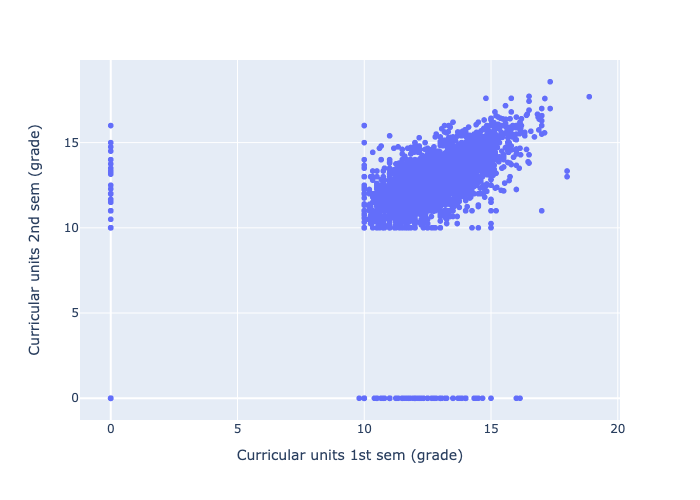
\includegraphics{report_AzadhdhinNedalYunisAlFraijat_files/figure-pdf/cell-51-output-1.png}

We can see that the points for the 1st semester and 2nd semester are
correlated which shows that are one's marks are primary drivers of
success and exhibit sizeable correlations

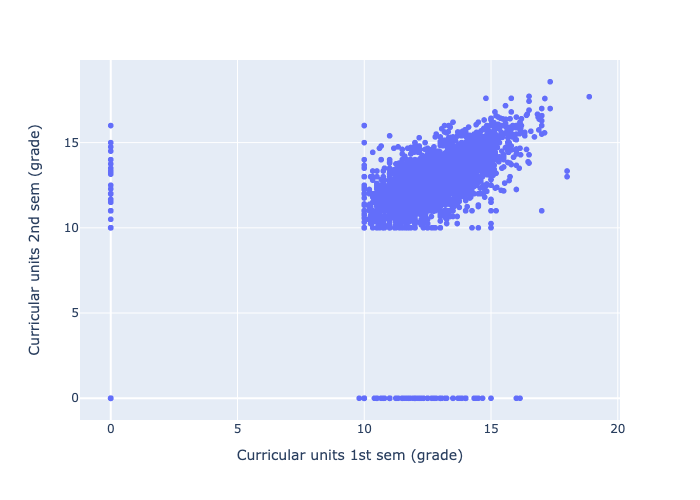
\includegraphics{report_AzadhdhinNedalYunisAlFraijat_files/figure-pdf/cell-52-output-1.png}

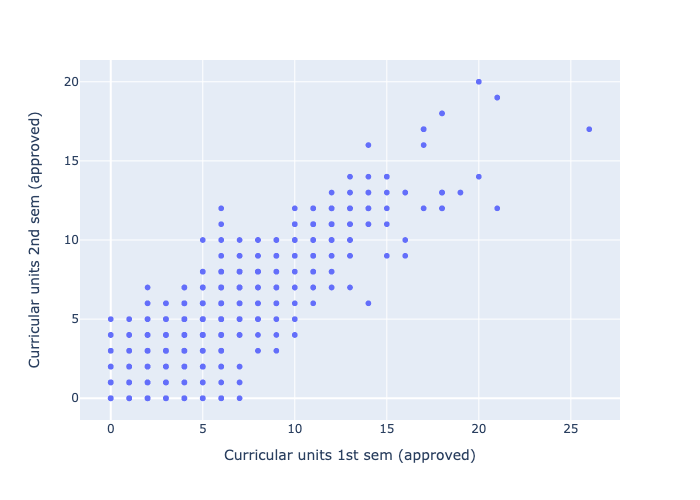
\includegraphics{report_AzadhdhinNedalYunisAlFraijat_files/figure-pdf/cell-53-output-1.png}

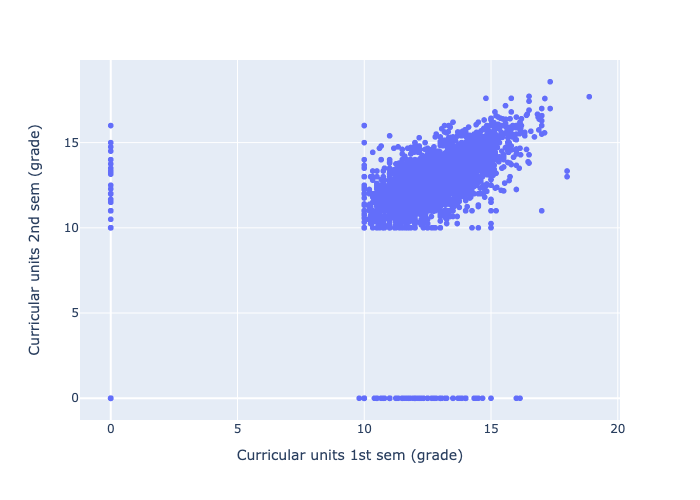
\includegraphics{report_AzadhdhinNedalYunisAlFraijat_files/figure-pdf/cell-54-output-1.png}

\hypertarget{data-mining}{%
\subsection{Data Mining}\label{data-mining}}

\hypertarget{conclusion}{%
\subsection{\texorpdfstring{\textbf{Conclusion}}{Conclusion}}\label{conclusion}}

\begin{quote}
With this analysis, we have some valuable insights some crucial factors
like Academic support, socioeconomic factors, previous qualifications,
and others play a significant role in student retention.
\end{quote}

\begin{quote}
The observed patterns imply a lot to stress in the lives of students and
their associates. First, we strive to insentivize parents to improve
their labour efficiency and pursue greater carreer so that ultimately
they could dedicate more time to their children's education, and
proactively stir their self-propelled interest. Additionally, we could
provide financial assistance to those who are struggling to pay with if
this is contemporaneous with a significant degradation in their
university marks, as this subrogates the stimuli for a person in an age
where they are most perceptive to knowledge and is a good predictor of a
dropout. Also importantly, we could teach the students, especially going
on their second studies, that it is quite unlikely that they are going
to get high grades or exit the university without proper time management
and confirmation that they assign top priority to their studies. They
are also advised to make that clear to all their relatives and
stakeholders who might underestimate the effects of such a change.
Although this could result in a reduction of enthusiastic entrants, this
would increase at least the KPI of retention and arguably also increase
the KPI on number of diplomas issued, because with fewer but more
motivated students the university would have more time to dedicate to
most obstinate pending alumni.
\end{quote}

\begin{quote}
Addressing these factors carefully can effectively lead to dropout rates
reduction and improve overall student outcomes
\end{quote}


\printbibliography


\end{document}
